\section{AG1: one selected-source homogeneous correction\workstar}
\subsection{The actual model and the term still outside this result}
After AI2's scoped admission, the advisor selected the homogeneous-update bottleneck. Work in the fixed energy unit $\delta=\alpha/8$ with the homogeneous reference
$G=H_0+\sum_bD_b$ and the actual selected S1 cubic-source family $A=\sum_b A_b$. Each $A_b$ is an identity-extended local mixing term on a complete four-factor star. It is a specified part of a repeated-anchor cubic contribution, not the entire cubic coefficient or transformed remainder. With $M=7|\tau|$, the available source norm satisfies
\begin{equation}
r_*:=\sup_b\norm{A_b}\le r_*^{\rm bd}
=\frac43\left(\frac7{12}\right)^{3/2}|\tau|^3.
\label{eq:cubic}
\end{equation}
Specifically, the inherited source is $A_b=|w_b\rangle\langle\Omega_b|+\mathrm{adjoint}$, where
\begin{equation}
v_b=\phi_b\Omega_b,\quad u_b=(H_{0,Z_b}|_{Q_b})^{-1}v_b,\quad
w_b=-\langle u_b,v_b\rangle u_b-\frac{\norm{u_b}^2}{3}v_b.
\label{eq:actualsource}
\end{equation}
The cubic expression in \eqref{eq:cubic} is an upper bound, not an evaluated equality. The frozen main interval is $0\le M\le10^{-3}$, with a predeclared refinement on $0\le M\le10^{-4}$. The auxiliary support-cardinality weight is $\rho=9/4$, while the required output uses the original weight two. These are proof parameters within the same homogeneous family; the filter time $T=3$ is not the canonical readout clock.

Translation of identical complete blocks gives the same actual norm $r=\norm{A_b}>0$ for every retained star when $\tau\ne0$. Deleting boundary stars does not modify a retained source. If $m_\Lambda$ is the maximum number of retained source stars containing a root, then $1\le m_\Lambda\le4$ for a nonempty family and its declared indexed norm is exactly
\begin{equation}
A_a:=\norm{\{A_b\}}_a=m_\Lambda a^4r,\qquad
\frac{A_\rho}{A_2}=\left(\frac98\right)^4.
\label{eq:denominator}
\end{equation}
This is a genuine input denominator even though $r$ is not numerically evaluated. Substituting its upper bound into a denominator would be invalid. Empty families and $\tau=0$ have zero update and are treated without division. Physical energies multiply these dimensionless bounds by $\delta$, with the original positive spacing and physical reference scales fixed.

If the full previously transformed Hamiltonian contains other terms $E$, the correct target remains $G+A+E$. Controlling $G+A$ does not control $E$. The exact equation below retains its transport and states the needed conditional norm premise. In particular AG1 is not a completed correction of every term in the original homogeneous Yang--Mills Hamiltonian.

\subsection{Domain-safe conjugation and the full nonlinear remainder}
For the triangular kernel $p_T(t)=(1-|t|/T)_+/T$ and its odd integrated primitive
$h_T(t)=\operatorname{sgn}(t)(1-|t|/T)^2/2$ on $0<|t|<T$, let
\begin{equation}
\mathcal R_T(A_b)=\int p_T(t)e^{itG}A_be^{-itG}\,dt,
\qquad
\mathcal J_T(A_b)=-i\int h_T(t)e^{itG}A_be^{-itG}\,dt.
\label{eq:filters}
\end{equation}
Their basic kernel identities are $h_T'=\delta_0-p_T$, $\int p_T=1$ and
$\int|h_T|=T/3$. Weak integration by parts gives a bounded commutator
$[\mathcal J_T(A_b),G]=-A_b+\mathcal R_T(A_b)$. The inherited adjoint-domain argument then gives graph-domain preservation. In a finite containing cuboid the sum $S=\sum_b\mathcal J_T(A_b)$ is bounded and skew-adjoint, preserves $D(G)$, and obeys
$[S,G]=-A+R$ with $R=\sum_b\mathcal R_T(A_b)$.

On that domain the exact update is
\begin{align}
e^S(G+A)e^{-S}&=G+R+N,\nonumber\\
N&=\sum_{n\ge1}\frac{\ad_S^n(nA+R)}{(n+1)!}
=\int_0^1e^{s\ad_S}\bigl(s[S,A]+(1-s)[S,R]\bigr)\,ds.
\label{eq:bch}
\end{align}
This identity expands the first commutator of $G$ only after replacing it by the bounded $-A+R$; all subsequent terms involve bounded interactions. To derive the coefficient, combine $\ad_S^nA/n!$ from the bounded $A$ conjugation with $\ad_S^n(-A+R)/(n+1)!$ from $G$. The result is $\ad_S^n(nA+R)/(n+1)!$. Thus the leading nonlinear term is $[S,A+R]/2$. A $G$-only BCH formula would omit a required contribution. The resonant filter residual is retained: the Fourier multiplier $\operatorname{sinc}^2(\omega T/2)$ equals one at zero frequency.

\subsection{Why the full commutator series needs weight loss}
For an indexed interaction with complete connected supports, define
\begin{equation}
\norm{\Phi}_a=\sup_x\sum_{X\ni x}a^{|X|}\norm{\Phi_X},\qquad a\ge2.
\label{eq:norm}
\end{equation}
Repeated terms with the same support retain their indices unless explicitly grouped. The forward complete rooted count starts at $N_0(a)=A_a$. Adding one interaction to a depth-$n$ connected word costs $2Ma^3$; the two root locations count stars meeting the existing union and incoming stars containing the root. This gives
\begin{equation}
N_{n+1}(a)\le8Ma^3(8+3n)N_n(a),\qquad
N_n(a)\le A_a(24Ma^3)^n(8/3)_n.
\label{eq:agcount}
\end{equation}
All ordered repetitions, incoming overlaps and complete supports remain. Finite boundaries only delete terms. The time simplex and exact kernel moments then give, with $x_a=72a^3M$ and $F_a=(1-x_a)^{-3}$,
\begin{align}
\norm R_a&\le A_a\sum_{n\ge0}\frac{2(8/3)_nx_a^n}{(n+2)!}\le A_aF_a,\nonumber\\
\norm S_a&\le A_a\sum_{n\ge0}\frac{6(8/3)_nx_a^n}{(n+3)!}\le A_aF_a.
\label{eq:agfilterbudget}
\end{align}
The last inequalities bound the entire positive orbital series of exponent $8/3$ by exponent three, using the unit absolute masses at $T=3$. At the main endpoint $x_\rho=6561/8000<1$, so these estimates hold continuously over the whole interval. The twelve interior crossings also preserve the inherited per-source residual bound $(24M+2/3)/(1-M)\le2072/2997$; that alone does not prove weighted-family contraction.

For $a>b\ge2$, overlap counting in a commutator has two possible root locations. After fixing one support, the overlapping second supports cost its cardinality. Nonempty overlap supplies a factor $b^{-1}\le1/2$, and
$\sup_{m\ge1}m(b/a)^m\le1/[e\log(a/b)]$ absorbs that cardinality. Therefore
\begin{equation}
\norm{[\Phi,\Psi]}_b\le
\frac{2}{e\log(a/b)}\norm{\Phi}_a\norm{\Psi}_a.
\label{eq:loss}
\end{equation}
Split the loss $\log(\rho/2)$ equally over $n$ commutators. Using
$n!\ge(n/e)^n$ gives
\begin{equation}
\frac{\norm{\ad_S^n X}_2}{n!}
\le\vartheta^n\norm{X}_\rho,\qquad
\vartheta=\frac{2\norm S_\rho}{\log(\rho/2)}
\le18\norm S_\rho,
\label{eq:nested}
\end{equation}
where $\log(9/8)\ge1/9$ gives the rational majorant. If a complete translated-source estimate proves a chosen upper bound $\bar\vartheta<1$, summing every BCH term yields
\begin{equation}
\norm N_2\le\frac{\bar\vartheta}{1-\bar\vartheta}
\left(\norm A_\rho+\frac12\norm R_\rho\right).
\label{eq:nonlinear}
\end{equation}
The complete rooted estimates, including repeated words, incoming overlaps and twelve possible interior crossings, are needed to justify the finite input norms. A finite-volume operator bound growing with $\norm{S_\Lambda}$ is not a substitute for a volume-independent interaction bound. Nor can the same positive weight margin be spent indefinitely without a new summable-loss induction.

For additional terms with a separately justified premise $\norm E_\rho\le e_*$,
\begin{equation}
e^S(G+A+E)e^{-S}=G+R+N+e^SEe^{-S},\qquad
\norm{e^SEe^{-S}}_2\le\frac{e_*}{1-\bar\vartheta}.
\label{eq:extra}
\end{equation}
The parameter $e_*$ is a conditional error inventory, not a fitted physical term. This inequality does not establish that the actual omitted $E$ satisfies it.

\subsection{The one-step estimates and the narrower contraction}
The forward rational majorant uses $r\le M^3/567$ and
$\bar\vartheta=72\rho^4F_\rho M^3/567$. At $M=10^{-3}$ it gives
$\bar\vartheta<5.5920\times10^{-7}$ and
\begin{equation}
\frac{\norm N_2}{A_2}\le\nu(M):=
\frac{\bar\vartheta}{1-\bar\vartheta}\left(\frac98\right)^4
\left(1+\frac{F_\rho}{2}\right)<7.7851\times10^{-5}.
\label{eq:nubudget}
\end{equation}
The underlying fractions, not the displayed rounding, establish the bound. Every positive factor increases with $M$ before its pole, so endpoint inequalities cover the continuous interval. This controls the whole nonlinear remainder, while the loose main residual majorant does not establish contraction there.

For $0<M\le10^{-4}$, split $R$ into its exact term without a $D_b$ interaction and the complete positive tail containing at least one $D_b$. On the original star the first part is
$|f_3(H_{0,Z_b})w_b\rangle\langle\Omega_b|+\mathrm{adjoint}$, where
$f_3(E)=\operatorname{sinc}^2(3E/2)$. The inherited source is orthogonal to the reference vacuum and its free local Hamiltonian has gap at least one. Thus $|f_3(E)|\le4/(9E^2)\le4/9$ on that source. The $n\ge1$ part of \eqref{eq:agfilterbudget} costs at most $A_2(F_2-1)$. Consequently
\begin{equation}
\frac{\norm{R+N}_2}{A_2}
\le\frac49+(1-576M)^{-3}-1+\nu(M)
<0.639242<\frac23.\workstar
\label{eq:contraction}
\end{equation}
This contracts against the actual chosen input norm \eqref{eq:denominator}, not two upper budgets. The independently derived reverse count uses different positive word majorants and gives the weaker bound $0.923603$ on the same interval. Post-exchange independent review verifies the stronger rooted recurrence used here. Unequal conservative constants are not conflicting evaluations of an exact observable. The narrower estimate is a predeclared refinement within AG1, not a fourth loop.

The skeptic separately retained more of the exact filter integration. With $\mathcal F(x)=(4-x)/(1-x)^2$, the positive $n\ge1$ tail has coefficient
$t(M)=\tfrac{16}{3}[\mathcal F(624M)-4]$ multiplying the actual $r_*$. The bound follows from the exact integrated coefficient
$32(4+3n)x^n/[(n+1)(n+2)]$ and $(n+1)(n+2)\ge6$. Since the actual input norm is at least $16r_*$, combining this tail with the skeptic's full nonlinear coefficient $n_{\rm sk}(M)$ gives
\begin{equation}
\frac{\norm{A'_{\rm new}}_2}{\norm A_2}
\le\frac49+\frac{t(M)+n_{\rm sk}(M)}{16}<0.605
\qquad(0<M\le10^{-4}).
\label{eq:skepticrefinement}
\end{equation}
This reviewer refinement, independently frozen and then cross-checked, improves a sufficient bound to about $0.604164$. The conservative reviewed headline remains one-step selected-source contraction below $2/3$. It is neither an exact dynamical contraction factor nor an extra physics loop.

\begin{figure}[ht]
\centering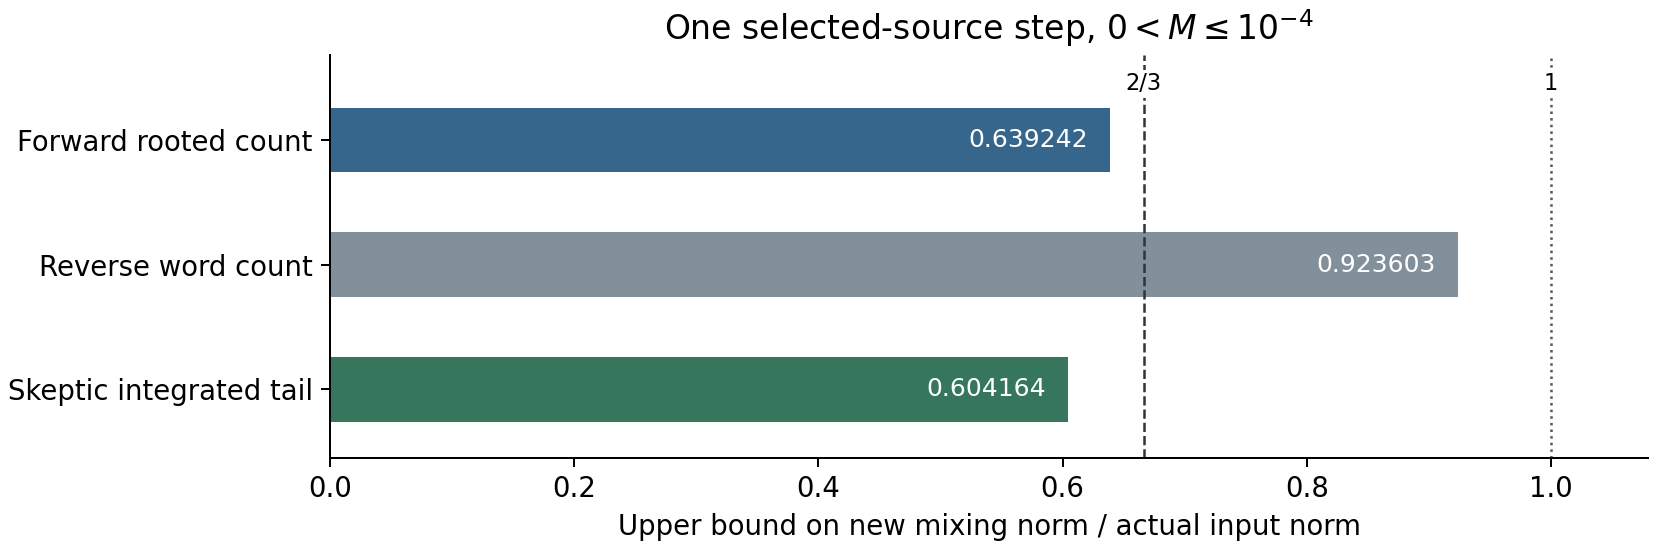
\includegraphics[width=.96\textwidth]{../../dist/ym-round27-contraction-bounds.png}
\caption{AG1 exact-output-backed sufficient bounds on the new selected mixing family, relative to the actual input norm. The producer bounds also cover $R+N$ before projection. Different positive-tail estimates produce different constants; none is an exact contraction measurement. The $2/3$ headline is supported by the reviewed forward and skeptic estimates.}
\end{figure}

For each generated self-adjoint indexed term $K_X$ of $K=R+N$, keep its full support and define $P_X=|\Omega_X\rangle\langle\Omega_X|$, $Q_X=I-P_X$ and
\begin{align}
c_X&=\langle\Omega_X,K_X\Omega_X\rangle,\quad
A'_X=P_XK_XQ_X+Q_XK_XP_X,\nonumber\\
D'_X&=Q_X(K_X-c_XI)Q_X,\qquad K_X=c_XI+A'_X+D'_X.
\label{eq:split}
\end{align}
The costs are $|c_X|\le\norm{K_X}$, $\norm{A'_X}\le\norm{K_X}$ and
$\norm{D'_X}\le2\norm{K_X}$, hence at most four times the budget when all three are summed. The scalar keeps its declared support for a density budget and may sum extensively. It is a reference expectation, not an interacting ground energy. ``Diagonal'' means the reference vacuum/complement split, not all excited spectral blocks. The new mixing family alone inherits \eqref{eq:contraction}; the changed diagonal, scalar and conditional $E$ cannot be discarded. The consumed weight margin, new supports and changed reference obstruct immediate iteration.

The checkers include both coupling signs, zero/empty cases, boundary multiplicities, all twelve crossings, complete positive tails, omitted-residual and wrong-BCH controls, scalar reconstruction and conditional $E$ transport. Independent finite rational matrix fixtures test algebraic coefficients; they are diagnostics, not the physical completeness proof. The all-order support and graph-domain arguments carry the result. The full original remainder inventory, all-stage induction, homogeneous numerical spectral gap, physical matching and continuum construction remain open.
